%!TEX root = ../Thesis.tex
\section{Paragraph2vec}

The pre trained word2vec model can't be used as basis for training the paragraph2vec model, as it don't contain the weights used in the hierarchical softmax, nor does it contain the structure of the Hoffman tree. Because of this both word and document vectors was trained.

The model was trained using the full text of all 273813 articles. The dimensionality of the word and document vectors was set to 500. Furthermore the model was trained over 10 epochs, with an initial learning rate of 0.025, which then decreased with 0.002 for each epoch. The vector representations of the chronologically first 100000 articles was then extracted from the final model.

Note that gensim doesn't provide any way of inspecting the loss function directly which is why no such curve is viewed here.  

\paragraph{Document vectors} Using principal component analysis the vector representations of all the documents can be visualized in both cases.

\begin{figure}[H]
	\centering
	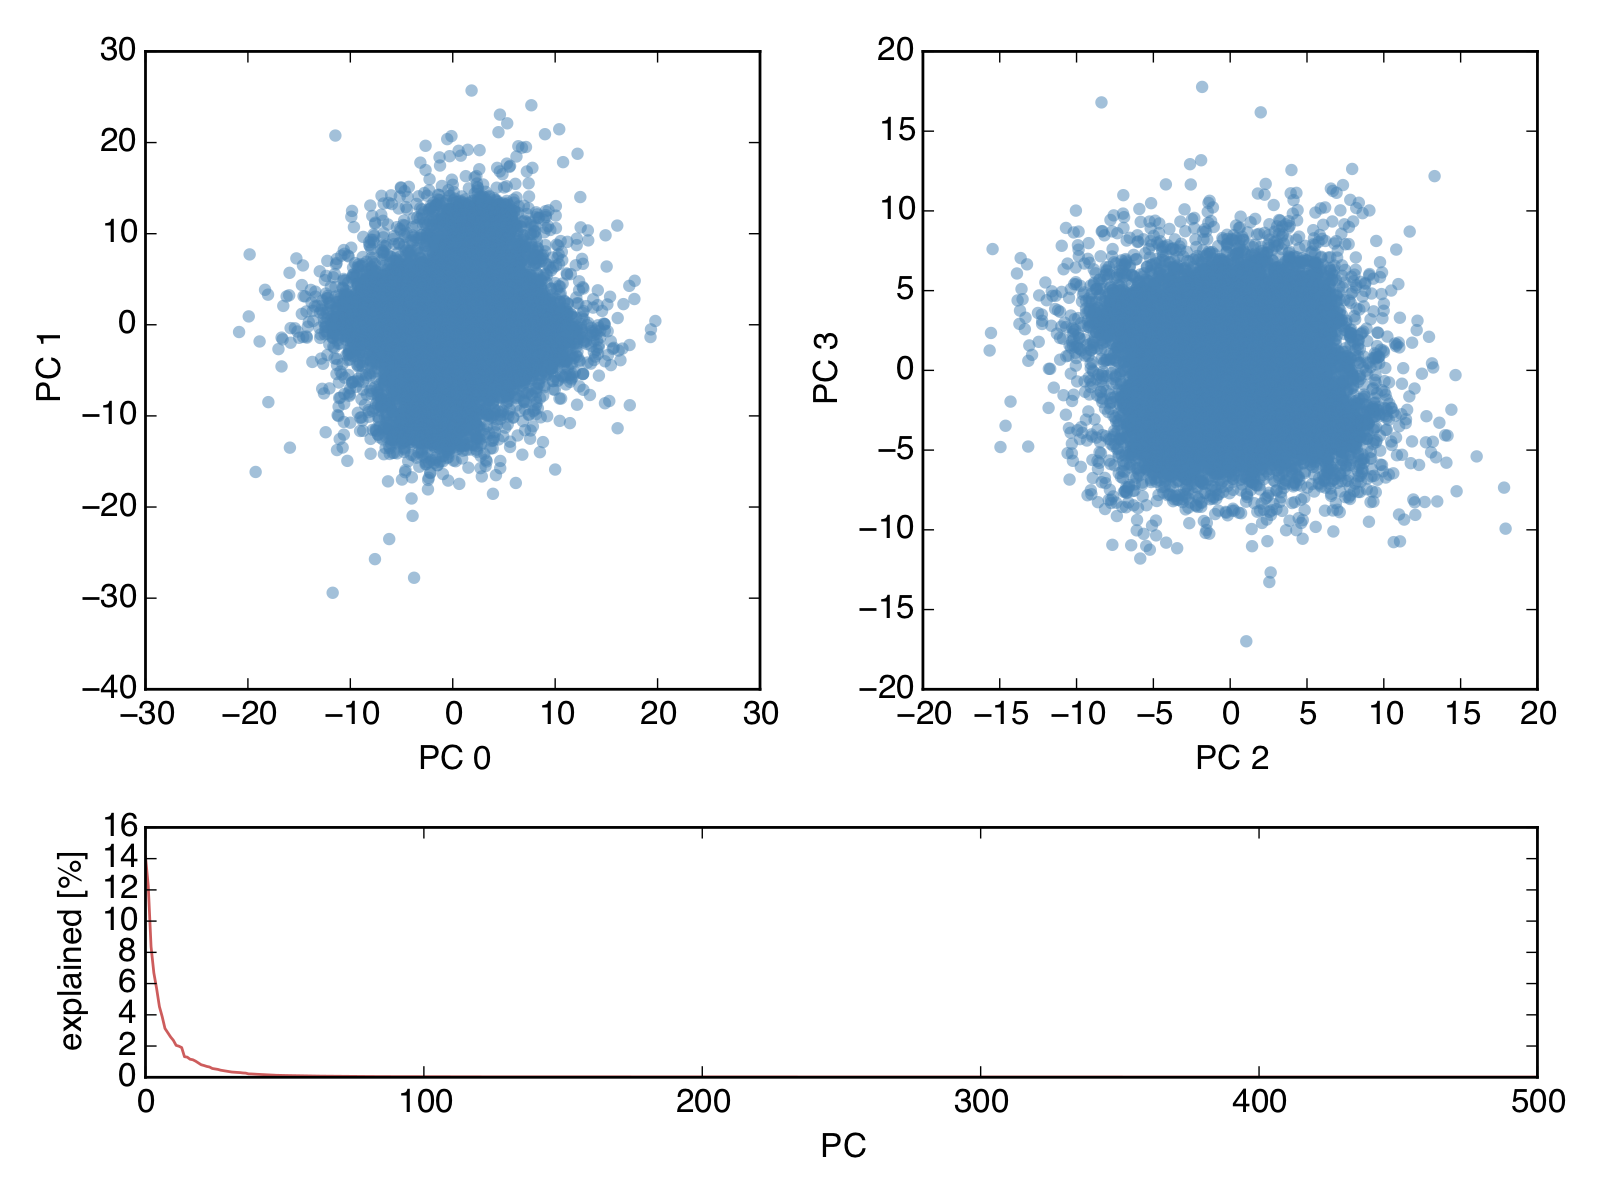
\includegraphics[width=0.9\textwidth]{results/doc2vec-pca}
	\caption{Document vectors calculated from just the title. Explaned variance on the first 4 principal components is 41.4\%.}
\end{figure}

Its quite interesting that 41.4\% of the variance is explained by the first 4 principal components. This might be because word2vec is quite good at guessing a missing word given just a short context. The big context which is what the document vector provides may very important and only inform about the general rhetorical pattern. This could be (formal versus  informal) or (angry versus happy). There thus exists a lower dimensional space there contains almost the same information as the 500 dimensional space.

\paragraph{Distance histogram} Again becase the distance is used for clustering, the distance histogram is inspected. Furthermore the $0.1\%$ percentile is used for calculating the threshold $t$.

\begin{figure}[H]
        \centering
        \begin{subfigure}[b]{0.49\textwidth}
                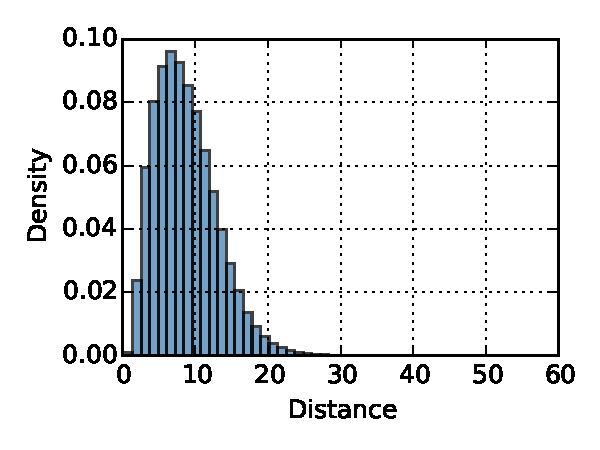
\includegraphics[width=\textwidth]{results/doc2vec-l2-histogram}
                \caption{Euclidian distance ($t \approx 1.35$)}
        \end{subfigure}
        \begin{subfigure}[b]{0.49\textwidth}
                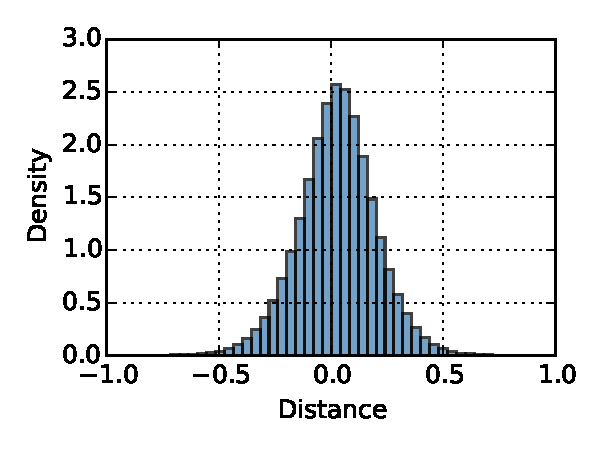
\includegraphics[width=\textwidth]{results/doc2vec-cos-histogram}
                \caption{Cosine similarity ($t \approx -0.66$)}
        \end{subfigure}
        \caption{Histograms of the distance, generating document vectors.}
\end{figure}

The distance histograms are distribution wise a bit cleaner than in the skip-gram case. This is likely because the distribution of the document is more multinormal, at least when inspecting the PCA plots. This will of cause result a cleaner distribution in the distance as well.

The euclidian distance distribution looks like a gamma distribution or similar. This is likely because of the squaring in the distance calculation, which prevents the distance from becoming negative. In the skip-gram case this was less of an issue because the mean (relative to the standard deviance) was larger.

\paragraph{Inspecting clusters} From inspecting the clusters the result seams to be worse when comparing to the skip-gram case.

When inspecting the cluster distribution it turns out that with paragraph2vec, clustering with cosine similarity actually yields more reasonably sized clusters, compared to when the euclidian distance is used for clustering. This may be because of the gamma like distribution of the euclidian distances, which makes it more difficult to separate articles about the same story from those about diffrent storries. It's possible that a more fine-tuned threshold could yield better results, but in any case there still exits too small and way too big clusters.

\begin{table}[H]
\centering
\begin{tabular}{r|l l l l l l l }
size & 1 & 2 & 3 & 421 & 711 & 1855 & 3326 \\ \hline
amount & 93665 & 8 & 2 & 1 & 1 & 1 & 1
\end{tabular}
\caption{The cluster distribution using an euclidan distance shows ureasonably large and small clusters and no reasonably or few reasonably sized clusters.}
\end{table}

Unfortunately the actual clusters that the clustering algorithm produces when using cosine similarity don't appear to capture any specific story. This is possibly because the document vectors only captures the overall mood of the article. For example the cluster in Table \ref{table:paragraph2vec:example} shows articles about some bad event.

At last it was checked if the ``teenage stowaway'' cluster existed in this case. This should be a fairly easy set of article to cluster as it contains very specific word combinations. Unfortunately it didn't as a single cluster, which again indicates the document vectors only tells about the overall mood of the document, as a way of adjusting the word probabilities.

\begin{table}[H]
\centering
\begin{tabular}{r|p{10cm}}
id & title \\ \hline
  9489 & Ukraine crisis: Draft document reveals sanctions against Russian and Crimean officials \\
  6644 & Six Nations 2014: Stuart Lancaster hints at unchanged England \\
  7573 & US opens emergency oil stockpile in signal to Putin \\
  8998 & Saudi Arabia bans 50 ‘blasphemous’ and ‘inappropriate’ children’s names \\
  7862 & Rangers: Recovery on track after title win - Ally McCoist
\end{tabular}
\caption{Cluster example when using cosine similarity on the paragraph2vec results.}
\label{table:paragraph2vec:example}
\end{table}
